\section{Incremental Table Maintenance} \label{sec:incremental_tabling}
%====================================================

\index{tabling!incremental}

XSB allows the user to declare that the system should maintain the
correctness of a given table with respect to dynamically changing
facts and rules through so-called {\em incremental
  tables}~\cite{SaRa05,Saha06,Swif14}.
%A table $T$ is {\em incremental} if XSB ensures that its answers are
%  consistent with all dynamic facts and rules upon which $T$ depends
%  (subject to transactionality conditions explained below).
After a database update or series of updates $\Delta$, an incremental
table $T$ that depends on $\Delta$ is by default updated
transparently: that is $T$ and all tables upon which $T$ depends are
automatically updated (if needed) whenever a future subgoal calls $T$.
%Alternately, if circumstances require it, a table can be updated
%immediately upon a database change or by issuing an explicit command
%to update all tables that depend on $\Delta$.
%
In either case, incremental tabling brings XSB closer to the
functionality of deductive databases.  If tables are thought of as
materialized database views (or snapshots), then the incremental table
maintenance subsystem enables incremental view maintenance; also as
discussed below, if choice points are thought of as database cursors
then incremental tabling also provides view consistency~\footnote{In
  the current version of XSB, there are certain restrictions on how
  incremental tabling can be used:
  cf. Section~\ref{sec:tabling-compatibility}.}.

\subsection{Transparent Incremental Tabling} \label{sec:incr_examples}

To demonstrate incremental table maintenance (informally called {\em
  incremental tabling}), consider first the following simple program
that does not use incremental tabling:
\begin{verbatim}
:- table p/2.
p(X,Y) :- q(X,Y),Y =< 5.

:- dynamic q/2.
q(a,1).    q(b,3).   q(c,5).    q(d,7).
\end{verbatim}
and the following queries and results:
\begin{verbatim}
| ?- p(X,Y),writeln([X,Y]),fail.
[c,5]
[b,3]
[a,1]

no
| ?- assert(q(d,4)).

yes
| ?- p(X,Y),writeln([X,Y]),fail.
[c,5]
[b,3]
[a,1]

no
\end{verbatim}
%
In this program, the table for {\tt p/2} depends on the contents of
the dynamic predicate {\tt q/2}.  We first evaluate a query, {\tt
  p(X,Y)}, which creates a table.  Then we use {\tt assert/1} to add a
fact to the {\tt q/2} predicate and re-evaluate the query.  We see
that the answers haven't changed, because the table is already created
and the second query just retrieves answers directly from that
existing table.  However the answers are inconsistent with the model
of {\tt p/2} after the assert.  I.e., if the table didn't exist
(e.g. if {\tt p/2} weren't tabled), the answer {\tt [d,4]} would also
be derived.  Without incremental table maintenance, the only solution
to this problem is for the XSB programmer to explicitly abolish a
table whenever changing (with assert or retract) a predicate on which
the table depends.
%
By declaring that the tables for {\tt p/2} should be incrementally
maintained, XSB automatically keeps the tables for {\tt p/2} correct.

%
Consider a slight rewrite of the above program:
\begin{verbatim}
:- table p/2 as incremental.
p(X,Y) :- q(X,Y),Y =< 5.

:- dynamic q/2 as incremental.
q(a,1).    q(b,3).    q(c,5).     q(d,7).
\end{verbatim}
in which {\tt p/2} is declared to be incrementally tabled
% (with {\tt  :- table p/2 as incremental}) 
and {\tt q/2} is declared to be both dynamic and incremental, meaning
that an incremental table depends on it.
%~\footnote{The declarations {\tt use\_incremental\_tabling/1} and
%  {\tt use\_incremental\_dynamic/1} are deprecated from Version 3.3 of
%  XSB forward -- in other words backwards compatibility will be
%  maintained for a time, but these declarations will not be further
%  supported.}.  
Consider the following goals and execution:
\begin{verbatim}
| ?- import incr_assert/1 from increval.
yes
| ?- p(X,Y),writeln([X,Y]),fail.
[c,5]
[b,3]
[a,1]

no
| ?- incr_assert(q(d,4)).

yes
| ?- p(X,Y),writeln([X,Y]),fail.
[d,4]
[c,5]
[b,3]
[a,1]

no
\end{verbatim}
\noindent
\index{Incremental Dependency Graph (IDG)}
\index{tabling!incremental!invalid subgoals}
The transparent approach to incremental updating works as follows.
When {\tt incr\_assert/1} is called, it sparks an invalidation
phase in which tables that depend on {\tt q(d,4)} are marked as {\em
  invalid} (i.e., possibly inconsistent with respect to underlying
dynamic code).  An {\em Incremental Dependency Graph (IDG)} is used to
obtain the right tables to invalidate.  However, if the invalidation
phase finds an affected table that is incomplete, a permission error
is thrown, since it is unclear whether sensible semantics can be given
to updating a subgoal that is incomplete.  After the invalidation
phase is completed, when/if a subgoal calls an invalid table $T$ the
engine interrupts itself to recompute $T$ and any tables upon which
$T$ depends.  On the other hand, if no calls are ever made to an
invalid incremental table $T'$, $T'$ will never incur the cost of an
update.

\index{view consistency}
\subsubsection{View Consistency} \label{sec:view-consistency}
%
As described above, transparent incremental tablings's use of lazy
updating ensures that a new query $Q$ will always be consistent with
the state of the dynamic code at the time $Q$ is called.  However,
transparent incremental tabling enforces a stronger property of view
consistency similar to those of database systems: that answers to a
query $Q$ should be those derivable at the time $Q$ was called, {\em
  and should not be affected by any updates}.
%Accordingly, the ISO standard for Prolog~\cite{ISO-Prolog} specifies
%that an update $\upsilon$ to dynamic code should not affect the
%behavior of choice points that were created before $\upsilon$.
Because XSB's incremental tabling does not allow updates that affect
tables that are still being computed, supporting view consistency
effectively means ensuring consistency for choice points into
completed incremental tables.  As such choice points correspond to
database cursors, we term them {\em Open Cursor Choice Points,
  (OCCPs)}.

XSB's support for view consistency is designed so that no perceptible
overhead in incurred if there are no OCCPs whose view needs to be
maintained.  Not surprisingly, numerous long-lived OCCPs whose views
need to be maintained across updates causes an overhead for the
engine, a situation that is in some sense similar to the cost of
maintaining views for cursors in database system.

%----------------------------------------------------------------
\comment{
In addition to the success continuations that are standard in most
languages, Prolog has failure continuations -- choice points to take
upon backtracking.  The presence of these failure continuations leads
to an issue of view consistency, even within a single-threaded
computation.  Suppose that a user
%
\begin{enumerate}
\item Makes a query to a completed incrementally tabled subgoal $Q$.
  $Q$ has more than one solution and the first one is returned,
  leaving a choice point into the table for $Q$.
\item Makes an update to dynamic code upon which $Q$ depends
\item Makes another query to $Q$
\end{enumerate}
%
What is the relation between the queries and the update.  Presumably,
the first query in step 1) should not reflect the changes made in step
2) if a user backtracks for further answers to that query -- this can
be seen as ensuring view consistency.. However it is less clear
whether the second query to $Q$ in step 4) should return the same
answers as the first query in step 1), or whether the second query
should reflect the database update.  Arguments can be made for either
approach.
%
\begin{itemize}
\item {\em Prolog-style semantics} If the second query reflects the
  database change, it is consistent with the database, but is not
  consistent with the first query~\footnote{This approach could be
    viewed as an extension of the ISO semantics for dynamic code in
    Prolog, which XSB does not currently support.};
\item {\em Delayed update semantics} If the second query does not
  reflect the dynamic code change, it is consistent with the first
  query but not with the dynamic code change.
\end{itemize}
%
XSB chooses the latter of these approaches.  If a user has failure
continuations into a query $Q$, then $Q$ and all tables that depend on
$Q$ will not be updated until these failure continuations have been
exhausted or removed.  However, all updates are ensured to be applied
once this is the failure continuations are removed.
}

%----------------------------------------------------------------

\subsection{Updating in a Three-Valued Logic}
%
As discussed earlier in this chapter, answers that are undefined in
the well-founded semantics are represented as conditional answers.
Beginning with version 3.3.7, incremental updates work correctly with
conditional answers~\footnote{Before Version 3.3.7, incremental
  updates only worked correctly on stratified tables: those with only
  unconditional answers.}.  Nno special care needs to be taken for
updating in the well-founded semantics as the following example
illustrates.
%conditional answers, and they can be updated through any of the
%previously described methods.  The following example illustrates one
%such approach.

\begin{verbatim}
:- dynamic data/1 as incremental.

:- table opaque_undef/0 as opaque.
opaque_undef:- tnot(opaque_undef).

:- table p/1 as incremental.
p(_X):- opaque_undef.
p(X):- data(X).
\end{verbatim}
%
Note that {\tt opaque\_undef/1} upon which {\tt p/1} depends is
explicitly declared as opaque~\footnote{An {\em opaque} predicate $P$
  is tabled and is used in the definition of some incrementally tabled
  predicate but should not be maintained incrementally.  In this case
  the system assumes that the programmer will abolish tables for $P$
  in such a way so that re-calling it will always give semantically
  correct answers.}.  When the above program is loaded, XSB will
behave as follows.
%
{\small
\begin{verbatim}
| ?- p1(1).

undefined
| ?- incr_assert(data(1)).

yes
| ?- p1(1).

yes
| ?- incr_retract(data(1)).

yes
| ?- p1(1).

undefined
| ?- get_residual(p1(1),C).

C = [opaque_undef]
\end{verbatim}
}
%

%\subsection{Eager Incremental Tabling}~\label{sec:incr-eager}
%%
%Despite the advantages of transparent incremental tabling, there are
%special circumstances when it may be better to update tables eagerly
%rather than when (and if) they are called.  For instance, if updates
%and queries are expected to occur at different times, performing eager
%updates may improve query time.  In addition, if incremental tables
%are accessed via table inspection predicates
%(cf. Chapter~\ref{sec:TablingPredicates}) rather than by queries,
%inconsistent answers may be obtained.  
%
%\paragraph{An Eager Updating Approach}
%%
%Usually, best way to eagerly update tables is to use the {\tt
%  incr\_assert/1} and {\tt incr\_retract(all)/1}
%predicates as discussed above.  When the updates are finished, the
%ommand {\tt incr\_table\_update/0} is then called, which updates all
%tables that depend on any changed dynamic rules or facts.  The
%following execution for our running program shows an example of this.

%\begin{verbatim}
%| ?- import incr_assert/1, incr_table_update/0 from increval.

%yes
%| ?- p(X,Y),writeln([X,Y]),fail.
%[c,5]
%[b,3]
%[a,1]
%%
%no
%| ?- incr_assert(q(d,4)), incr_assert(q(d,1)), 
%
%yes
%| ?- incr_table_update.
%
%| ?- p(X,Y),writeln([X,Y]),fail.
%[d,4]
%[d,1]
%[c,5]
%[b,3]
%[a,1]
%
%no
%\end{verbatim}
%\noindent
%As discussed, calling {\tt incr\_table\_update} causes the cost of
%updating incremental tables to be immediately incurred, and ensures
%that table inspection primitives show correct results.  However,
%tables are updated and their views preserved even if the tables may
%not be accessed before further updates are made.
%
%\paragraph{Issues with Eager Updating}
%%
%In the current version of XSB, eager updating is taken to be something
%of a special use case.  In order to perform eager updating, a global
%update list is maintained whenever changes are made to incremental
%dynamic predicates or tries.  In particular, the list is not updated
%when incremental tables are abolished, so that if an incremental table
%has been abolished making the global update list possibly invalid,
%%eager updating will be disabled for the rest of the session (unless
%{\tt abolish\_all\_tables/0} is called.  In this state, a call to {\tt
%  incr\_table\_update} will throw a permission error.

%\subsubsection{An Immediate Approach}
%
%A final approach is to use the predicates {\tt incr\_assert\_immed/1}
%and {\tt incr\_retract(all)\_immed/1}, which force immedidate updates
%of invalidated tables.  While simple, this approach should only be
%used in special circumstances, as calling {\tt incr\_assert\_update/1}
%twice could cause tables to be updated twice rather than once.
%
%\comment{
% We note, however, that the use of these predicates is much
%less common than direct queries to tables; but if using table
%inspection predicates on incrementally maintained tables, the user
%should ensure that the tables have been eagerly updated as described
%below in Section~\ref{}.  should ensure that {\tt
%  incr\_table\_update/0} is called before inspecting the tables.
%
%Here again we call {\tt p(X,Y)} and generate a table for it and its
%answers.  Then we update {\tt q/2} by using the incremental version of
%%assert, {\tt incr\_assert/1}, which was explicitly imported.  Now when
%we call {\tt p(X,Y)} again, the table has been updated and we get the
%correct answer.
%
%In this case after every {\tt incr\_assert/1} and/or {\tt
%  incr\_retract(all)/1}, the tables are incrementally updated to
%reflect the change.  The system keeps track of what tabled goals
%depend on what other tabled goals and (incremental) dynamic goals, and
%tries to minimize the amount of recomputation necessary.
%Incrementally tabled predicates may depend on other tabled predicates.
%In this case, those tabled predicates must also be declared as
%incremental (or opaque).The algorithm used is described
%in~
%}
\subsubsection{Declaring Predicates to be Incremental}
%
In XSB, tables can have numerous properties: such as {\em subsumptive,
  variant, incremental, opaque, dynamic, private}, and {\em shared},
and can use answer subsumption, answer abstraction or call
abstraction.  XSB also has variations in forms of dynamic predicates:
{\em tabled, incremental, private}, and {\em shared}.  XSB extends the
{\tt table} and {\tt dynamic} compiler and executable directives with
modifiers that allow users to indicate the kind of tabled or dynamic
predicate they want.  For example,
%
\begin{verbatim}
:- table p/3,s/1 as subsumptive,private.

:- table q/3 as incremental,variant.

:- dynamic r/2,t/1 as incremental.
\end{verbatim}
%We note that
%\begin{verbatim}
%:- table p/3 as dyn.
%and
%:- dynamic p/3 as tabled.
%\end{verbatim}
%are equivalent.

In the current version of XSB, incremental tabling works with subgoal
abstraction, answer abstraction, and well-founded negation.  However
several combinations involving incremental tabling are not supported
and will throw an error (cf. page \pageref{table-declaration} and page
\pageref{dynamic-declaration}, respectively). Incremental tabling has
not yet been ported to the multi-threaded engine and it currently does
{\em not} works for predicates that use call subsumption or answer
subsumption.

\index{tries!and incremental tabling}
\subsection{Incremental Tabling using Interned Tries} \label{sec:incr-update-tries}
%
Sometimes it is more convenient or efficient to maintain facts in
interned tries rather than as dynamically asserted facts
(cf. Chapter~\ref{chap:tries}).  Tables based on interned tries can be
automatically updated when terms are interned or uninterned just as
they can be automatically updated when a fact is asserted or
retracted.  Consider the example from Section~\ref{sec:incr_examples}
rewritten to use interned tries.  As usual, an incrementally updated
table is declared as such:
%
\begin{verbatim}
:- table p/2 as incremental.
\end{verbatim}
%
However, the declaration for dynamic data changes: rather than using
the declaration 
\begin{center}
{\tt :- dynamic q/2 as incremental}
\end{center}
a trie is specified as incremental in its creation.
%
\begin{center}
{\tt  trie\_create(Trie\_handle,[incremental,alias(inctrie)])}
\end{center}
%
As described in Chapter~\ref{chap:tries}, the trie handle returned is
an integer, but can be aliased just as with any other trie.  The trie
may then be initially loaded:
%
\begin{verbatim}
	trie_intern(q(a,1),inctrie),trie_intern(q(b,3),inctrie),
	trie_intern(q(c,5),inctrie),trie_intern(q(d,7),inctrie).
\end{verbatim}
%
At this stage a query to {\tt p/2} acts as before:
%
\begin{verbatim}
p(X,Y) :- trie_interned(q(X,Y),inctrie),Y =< 5.

| ?- p(X,Y),writeln([X,Y]),fail.
[c,5]
[b,3]
[a,1]
\end{verbatim}
%
The following sequence ensures that {\tt p/2} is incrementally updated
as {\tt inctrie} changes:
%
\begin{verbatim}
| ?- import incr_trie_intern/2.

yes
| ?- incr_trie_intern(inctrie,q(d,4)).

yes
| ?- p(X,Y),writeln([X,Y]),fail.
[d,4]
[c,5]
[b,3]
[a,1]

no
\end{verbatim}
%
Given the proper directives to make a trie incremental, transparent
incremental tabling works for changes made to interned tries just as
it does for regular dynamic code and for trie-indexed dynamic code.
%There are also the predicates {\tt incr\_trie\_intern\_update/2} and
%{\tt incr\_trie\_unintern\_updatesl/2} which immediately update
%dependent tables.

\index{Incremental Dependency Graph (IDG)}
\subsection{Abstracting the IDG for Better Performance} \label{sec:IDG-abs}
As mentioned above, incremental table maintenance makes use of an IDG.
Specifically, the nodes of the IDG are the incrementally tabled
subgoals; and each such table contains information about its incident
edges: those subgoals upon which a node directly depends or directly
affects.  While the IDG is a critical data structure to efficiently
update incremental tables, in certain situations constructing the IDG
can cause non-trivial overheads in query time and table space.  These
overheads can be addressed in many cases by {\em abstracting} the IDG.
When a tabled subgoal $S$ is called, rather than creating an edge
between $S$ and its nearest tabled ancestor $S'$ (if any), one could
abstract $S$, $S'$ or both, potentially collapsing a large number of
nodes and edges of the IDG.  If $S$ is an incremental table, then
performing subgoal abstraction on $S$ as introduced in
Section~\ref{sec:tabling-termination}, will abstract the IDG -- rather
than having $n$ nodes $S_1,\ldots,S_n$ and their associated links, the
IDG will contain a single node $abstract(S)$.  However, subgoal
abstraction will not work to abstract the leaf nodes of the IDG, which
are subgoals to non-tabled dynamic incremental predicates.

In \version{} of XSB, IDG nodes for dynamic incremental predicates may
undergo depth abstraction: given a subgoal $S$ and integer $k$,
subterms of $S$ with depth $k+1$ are replaced by unique new variables.
For instance, abstracting
%the term 
{\em q(f(1))} at level 1 gives {\em q(f(X$_1$))}; abstracting at level
0 gives {\em q(X$_1$)}.
%
Figure~\ref{fig:abstraction} illustrates an important case where
abstracting dynamic incremental predicates can be critical to good
performance for incremental tabling.  In the case of left-linear
recursion, if no abstraction is used a new node will be created for
each call to {\tt edge/2} as shown on the left side of this figure.
If a large number of data elements are in fact reachable, the size of
the IDG can be very large.  If calls to the {\tt edge/2} predicate
make use of depth-0 abstraction, the graph may be much smaller as seen
on the right side of Fig.~\ref{fig:abstraction}.  Whether abstracting
a IDG in this manner is useful or not is application dependent;
however, performance results indicate that for left-linear recursion,
abstraction greatly reduces both query time and space.

%------------------------------------------------------------
\begin{figure}[ht]
\centering
\begin{minipage}[b]{0.25\linewidth}
{\tt
\begin{tabbing}
fooofoofoofoofoofoofoofooooooooooooooooooooooooooo\=ooooooooooooo\=\kill
:- table reach/2 as incremental.\\
:- dynamic edge/2 as incremental.\\
reach(X,Y):- edge(X,Y). \\
 reach(X,Y):- reach(X,Z),edge(Z,Y). \\
\end{tabbing}
}
\end{minipage}
%\quad
\begin{minipage}[b]{0.25\linewidth}
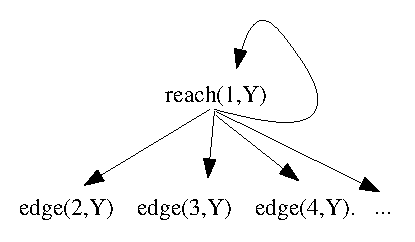
\includegraphics[width=\textwidth]{recursion}
%  \caption{Without \abstraction}
%  \label{fig:minipage1}
\end{minipage}
\quad
\begin{minipage}[b]{0.25\linewidth}
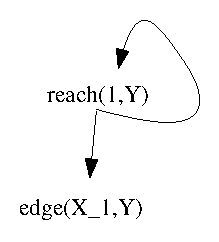
\includegraphics[width=0.5\textwidth]{abs-recursion}
%  \caption{With \abstraction}
%  \label{fig:minipage2}
\end{minipage}
\caption{A left-linear program and schematic IDGs: Left
  without IDG abstraction; Right: with
  IDG abstraction} \label{fig:abstraction}
\end{figure}
%------------------------------------------------------------
Abstracting the {\tt edge/2} predicate has subtle differences from
abstracting tabled subgoals.
%  The implementation of subgoal
%abstraction for tabled subgoals was described in~\cite{RigS13},
As mentioned, the {\tt edge/2} predicate of
Fig.~\ref{fig:abstraction} is not tabled.  Furthermore, the actual
{\tt edge/2} subgoal itself should not be abstracted to depth 0 since
losing the first argument instantiation would prevent the use of
indexing.  Rather, only the IDG's representation of the subgoal
should be abstracted.  Abstraction of dynamic code for
the IDG can be specified via the declaration:
\begin{center}
{\tt :-dynamic edge/2 as incremental, abstract(0)}.
\end{center}

In \version{} dynamic incremental code can be abstracted, but
incremental interned tries (Section~\ref{sec:incr-update-tries})
cannot be.  Also, currently only depth 0 abstraction is supported.

\subsection{Summary and Implementation Status}
%
%When using incremental tabling, an application will most commonly need
%only the default transparent approach, although in special
%circumstances eager updating may be desired.  

The main design choices of incremental tabling
are as usual what to table, and also what dynamic predicates or tries
should be made incremental.  In addition, performance optimizations
may be made through a mixture of subgoal abstraction and dynamic
predicate abstraction.  This optimization can be informed by use of
{\tt statistics/0} which includes summary information about the IDG,
or using the IDG inspection predicates of
Section~\ref{sec:incr-preds1} if more details are needed.

%Thus the user has four choices: tables may be
%updated as soon as the database is changed (e.g., via {\tt
%  incr\_assert/1}); at some point after a series of database changes
%(e.g. via {\tt incr\_assert\_inval/1} and {\tt
%  incr\_table\_update/0}); or lazily whenever a given table is called.
%In addition, if the changes are so massive that there is no point in
%incrementally updating the table, the tables can be abolished so that
%the tables will be reconstructed whenever they are re-queried.

In the current version of XSB, incremental tabling has not yet been
ported to the multi-threaded engine.  In addition, incremental tabling
only works for predicates that use both call and answer variance.
However, incremental tabling does work with for the full well-founded
semantics, for trie indexed dynamic code (in addition to regular
dynamic code) and with interned tries as described in
Section~\ref{sec:incr-update-tries}.  The space reclamation predicates
{\tt abolish\_all\_tables/0}, {\tt abolish\_table\_call/[1,2]} and
{\tt abolish\_table\_pred/[1,2]} can be safely used with incremental
tables.

\subsection{Predicates for Incremental Table Maintenance} \label{sec:incr-preds1}

\paragraph{A Note on Terminology}
%
Suppose {\tt p/1} and {\tt q/1} are incrementally tabled, and that
there is a clause
%
\begin{verbatim}
p(X):- q(X).
\end{verbatim}
%
In this case we say that {\tt p(X)} {\em depends\_on} {\tt q(X)} and
that {\tt q(X)} {\em affects} {\tt p(X)}.  A recursive predicate both
depends on and affects itself.


\paragraph{Declarations} The following directives support incremental
tabling based on changes in dynamic code: 

\index{tabling!opaque}
\index{tabling!declarations}
\begin{description}
\index{tabling!incremental}

\ourstandarditem{table +PredSpecs as incremental}{table/1}{Tabling}
%
is a executable predicate that indicates that each tabled predicate
specified in {\tt PredSpec} is to have its tables maintained
incrementally.  {\tt PredSpec} is a list of skeletons, i.e. open
terms, or {\tt Pred/Arity} specifications~\footnote{No explicit module
  references are allowed.}.  The tables must use call variance and
answer variance and must be compiled and loaded into the
single-threaded engine.  If a predicate is declared with tabling
attributes that are not supported with incremental tabling a
permission error is thrown.  This predicate implies that its arguments
are tabled predicates.  See page \pageref{table-declaration} for
further discussion of tabling options.

We also note that any tabled predicate that is called by a predicate
tabled as incremental must also be tabled as incremental or as opaque.
On the other hand, a dynamic predicate {\tt d/n} that is called by a
predicate tabled as incremental may or may not need to be declared as
incremental.  However if {\tt d/n} is not declared incremental, then
changes to it will not be propagated to incrementally maintained
tables.

\ourstandarditem{dynamic +PredSpecs as incremental}{dynamic/1}{Tabling}
%
is an executable predicate that indicates that each predicate in {\tt
  PredSpecs} is dynamic and used to define an incrementally tabled
predicate and will be updated using {\tt incr\_assert/1} and/or {\tt
  incr\_retractall/1} (or relatives.)  Note that dynamic incremental
predicates cannot themselves be tabled.  This predicate implies that
its arguments are dynamic predicates.  See page
\pageref{dynamic-declaration} for further discussion of dynamic
options.

\ourstandarditem{table +PredSpecs as opaque}{table/1}{Tabling} 
%
is an executable predicate that indicates that each predicate $P$ in
{\tt PredSpecs} is tabled and is used in the definition of some
incrementally tabled predicate but should not be maintained
incrementally.  In this case the system assumes that the programmer
will abolish tables for $P$ in such a way so that re-calling it will
always give semantically correct answers.  In other words, instead of
maintaining information to support incremental table maintenance, the
system re-calls the opaque predicate whenever its results are required
to recompute an answer.  One example of an appropriate use of opaque
is for tabled predicates in a DCG used to parse some string.  Rather
than incrementally maintain all dependencies on all input strings, the
user can declare these intermediate tables as opaque and abolish them
before any call to the DCG.  This predicate implies that its arguments
are tabled predicates.

\end{description}

\paragraph{Basic Incremental Maintenance Predicates}
The following predicates are used to manipulate incrementally
maintained tables:

\begin{description}
\ourrepeatmoditem{incr\_assert(+Clause)}{incr\_assert/1}{increval} 
\ourrepeatmoditem{incr\_assertz(+Clause)}{incr\_assertz/1}{increval}
\ourrepeatmoditem{incr\_asserta(+Clause)}{incr\_asserta/1}{increval}
\ourrepeatmoditem{incr\_retract(+Clause)}{incr\_retract/1}{increval}
\ourmoditem{incr\_retractall(+Term)}{incr\_retractall/1}{increval}
% 
are versions of {\tt assert/1} and other standard Prolog predicates.
They modify dynamic code just as their Prolog counterparts, but they
first invalidate all incrementally maintained tables that depend on
{\tt Clause}.

{\bf Error Cases} are the same as {\tt assert<a/z>/1}, {\tt retract/1}
and {\tt retractall/1} with the additional error conditions that
relate to the semantics of incremental tabling.  Note that if these
error conditions arise, the update will {\tt not} occur.

\begin{itemize}
\item The head of the clause {\tt Clause} or the {\tt Term} refers to
  a predicate that is not incremental and dynamic.  
\bi
\item  {\tt type error(dynamic\_incremental, Term)}
\ei
%
\item {\tt Clause} affects an incremental table that is incomplete
  (and so is in the course of being computed).
\bi
\item  {\tt permission\_error}
\ei 
\end{itemize}

%\ourrepeatmoditem{incr\_assert\_immed(+Clause)}{incr\_assert\_immed/1}{increval}
%\ourrepeatmoditem{incr\_assertz\_immed(+Clause)}{incr\_assertz\_immed/1}{increval}
%\ourrepeatmoditem{incr\_asserta\_immed(+Clause)}{incr\_asserta\_immed/1}{increval}\
%\ourrepeatmoditem{incr\_retractall\_immed(+Clause)}{incr\_retractall\_immed/1}{increval}
%\ourmoditem{incr\_retract\_immed(+Term)}{incr\_retract\_immed/1}{increval}
%%
%are versions of {\tt assert/1} and other standard Prolog predicates.
%They modify dynamic code just as their Prolog counterparts, mark any
%incrementally maintained tables that depend on the modification as
%invalid, then immediately update these tables.
%%  The tables may be updated by an
%explicit call to {\tt incr\_table\_immed/[0,1,2]}, or the table will
%be dynamically recomputed when a query is made to it.

%\ourmoditem{incr\_table\_update}{incr\_table\_update/0}{increval} may
%be called after base predicates have been changed (by {\tt
%  incr\_assert/1} and/or {\tt incr\_retract/1} or friends).  This
%predicate updates all the incrementally maintained tables whose
%contents may be affected by those changes to the base predicates.
%This update operation is separated from the operations that change the
%base predicates ({\tt incr\_assert\_inval/1} and {\tt
%  incr\_retractall\_inval/1}) so that a set of base predicate changes
%can be processed all at once, which may be much more efficient that
%updating the tables at every base update.  Beginning with Version
%3.3.7, it is not absolutely necessary to call this predicate, as
%tables will be incrementally updated upon demand.  However, using this
%predicate allows a choice of incurring the cost of update at a time
%other than querying an updated goal.
%Explicit update calls only need to be used in special circumstances
%(cf. Section~\ref{sec:incr-eager}).

%{\bf Error Cases}
%\bi
%\item A table $T$ that is to be incrementally updated is not yet
%  complete.  
%\bi
%\item 	{\tt permission\_error(update, incomplete\_table Goal)}
%\ei
%\item An abolish of some incremental table has made the global update
%  list potentially corrupted.
%\bi
%\item {\tt permission\_error}
%\ei 
%  \ei

%\ourmoditem{incr\_table\_update(-GoalList)}{incr\_table\_update/1}{increval}
%acts as {\tt incr\_table\_update/0} in its action to update the
%incrementally maintained tables after changes to base predicates.  It
%returns the list of goals whose tables were changed in the update
%process.
%
%\ourmoditem{incr\_table\_update(+SkelList,-GoalList)}{incr\_table\_update/2}{increval}
%acts as {\tt incr\_table\_update/1} in its action to update
%incrementally maintained tables after changes to base predicates.  The
%first argument is a list of predicate skeletons (open terms) for
%incrementally maintained tables.  The predicate returns in {\tt
%  GoalList} a list of goals whose skeletons appear in {\tt SkelList}
%and whose tables were changed in the update process.  In this way {\tt
%  SkelList} acts as a filter to restrict the goals that are returned
%to those of interest.  If {\tt SkelList} is a variable, all affected
%goals are returned in {\tt GoalList}.

\ourmoditem{incr\_invalidate\_call(+Goal)}{incr\_invalidate\_call/1}{increval}
Let $\cT$ be the least set of all incrementally maintained tables
whose goals that unify with {\tt Goal}, or whose tables are
(transitively) affected by a goal in $\cT$.  This predicate invalidates
all tables in $\cT$.  Any subsequent call to a goal $G$ associated
with $\cT$ will be automatically be incrementally updated if
necessary.  (As will any goals that $G$ depends on that are in need of
updating.)  In a similar manner, an invocation of {\tt
  incr\_table\_update/[0,1,2]} will cause tables in $\cT$ to be
updated.

Note that this predicate is needed for exceptional cases only.  Calls
to {\tt incr\_assert/1} and similar predicates mentioned above perform
invalidation automatically, as does {\tt abolish\_table\_call/[1,2]}.
However, {\tt incr\_invaldate\_calls/1} is useful if a tabled
predicate depends on some external data and not (only) on dynamic
incremental predicates.  For example, such a predicate might depend on
a relation stored in an external relational database (perhaps accessed
through the ODBC interface).
% then this predicate can be used to invalidate the
%table when the external relation changes.  
Of course, in such a case, the application programmer must know when
the external relation changes and invoke {\tt
  incr\_invalidate\_calls/1} as necessary.


{\bf Error Cases}
\bi
\item 	{\tt Goal} is tabled, but not incrementally tabled
\bi
\item 	{\tt permission\_error(invalidate,non-incremental predicate,Goal)}
\ei
\ei

\end{description}

\paragraph{Incremental Maintenance using Interned Tries}
The following predicates are used to modify incremental tries, and can
be freely intermixed with predicates for modifying incremental dynamic
code, as well as with predicates for invalidating or updating tables
(Section~\ref{sec:incr-preds1}).

\begin{description}
\ourmoditem{incr\_trie\_intern(+TrieIdOrAlias,+Term)}{incr\_trie\_intern/2}{intern}
%
is a version of {\tt trie\_intern/2} for tries declared as
incremental.  A call to this predicate interns {\tt Term} in {\tt
  TrieIdOrAlias} and then invalidates all incrementally maintained
tables that depend on this trie.

\ourmoditem{incr\_trie\_uninternall(+TrieIdOrAlias,+Term)}{incr\_trie\_uninternall/2}{intern}
%
is a version of {\tt trie\_unintern/2} for tries declared as
incremental.  A call to this predicate removes all terms unifying with
{\tt Term} in {\tt TrieIdOrAlias} and then invalidates all
incrementally maintained tables that depend on this trie.

%\ourmoditem{incr\_trie\_intern\_immed(+TrieIdOrAlias,+Term)}
%           {incr\_trie\_intern\_immed/2}{intern}
%%
%works for tries declared as incremental in a similar manner as {\tt
%  incr\_trie\_intern/2} except that it also immediatesly updates any
%affected tables.

%\ourmoditem{incr\_trie\_uninternall\_immed(+TrieIdOrAlias,+Term)}
%{incr\_trie\_uninternall\_immed/2}{intern}
%
%works for tries declared as incremental in a similar manner as {\tt
%  incr\_trie\_uninternall/2} except that it also immediately updates
%any affected tables.
\end{description}

\index{residual dependency graph}
\index{Incremental Dependency Graph (IDG)}
\paragraph{Inspecting the State of the Incremental Dependency Graph}
%
% These relations form a labelled directed graph for which the
%nodes are incrementally tabled subgoals present in XSB; a given
%subgoal in the graph may or may not have been completed.  
%Conceptually, there is an edge from $S_1$ to $S_2$ labelled depends
%(affects) if $S_1$ directly depends on (directly affects) $S_2$.  We
%call this graph the {\em incrementally tabled subgoal dependency
%  graph}, or just the incremental dependency graph.  
The predicates in this section allow a user to inspect properties of
IDG that can be useful in debugging, profiling or optimizing a
computation~\footnote{The predicates for traversing the incremental
  dependency graph are somewhat analogous to those for traversing the
  residual dependency graph (Section~\ref{sec:table-inspection}).}.
In addition they provide information about which subgoals in the IDG
are invalid -- i.e., which subgoals depend on a dynamic code that has
changed, but have not been updated.

As explained below, IDG nodes can be accessed via the predicate {\tt
  is\_incremental\_subgoal/1}, while IDG edges can be accessed via
{\tt incr\_directly\_depends/2}.  The predicates {\tt
  get\_incr\_scc/[1,2]} and {\tt get\_incr\_scc\_with\_deps/[3,4]} can
be used to efficiently materialize the dependency graph in Prolog,
including SCC information.  Similarly, the predicate {\tt
  subgoal\_property/2} can be used to determine which subgoals are
invalid.

\begin{description}

\ourmoditem{is\_incremental\_subgoal(?Subgoal)}{is\_incremental\_subgoal/1}{increval}
%
This predicate non-deterministically unifies {\tt Subgoal} with
incrementally tabled subgoals that are currently table entries.

\ourmoditem{incr\_directly\_depends(?Goal$_1$,?Goal$_2$)}{incr\_directly\_depends/2}{increval}
accesses the edges of the IDG: the incremental goals (Tables) that
directly depend on or directly affect one another.  At least one of
{\tt Goal$_1$} or {\tt Goal$_2$} must be bound.
\begin{itemize}
\item If {\tt Goal$_1$} is bound, then this predicate will return in
  {\tt Goal$_2$} through backtracking the goals for all incrementally
  maintained tables and dynamic leaf nodes on which {\tt Goal$_1$}
  directly depends.
\item If {\tt Goal$_2$} is bound, then it returns in {\tt Goal$_1$}
  through backtracking the goals for all incrementally maintained
  tables that {\tt Goal$_2$} directly affects -- in other words all
  goals that directly depend on {\tt Goal$_2$}.  \ei

{\bf Error Cases}
\bi
\item Neither {\tt Goal$_1$} nor {\tt Goal$_2$} is bound 
\bi
\item 	{\tt instatiation\_error}
\ei
\item {\tt Goal$_1$} and/or {\tt Goal$_2$} is bound, but is not
  incrementally tabled
\bi
\item 	{\tt table\_error}
\ei
\ei

\ourmoditem{incr\_trans\_depends(?Goal$_1$,?Goal$_2$)}{incr\_trans\_depends/2}{increval}
is similar to {\tt incr\_directly\_depends/2} except that it returns
goals according to the transitive closure of the ``directly depends''
relation.  Error conditions are the same as {\tt
  incr\_directly\_depends/2}.

\ourrepeatmoditem{get\_incr\_sccs(?SCCList)}{get\_incr\_sccs/1}{increval}
\ourrepeatmoditem{get\_incr\_sccs\_with\_deps(?SCCList,?DepList)}{get\_incr\_sccs\_with\_deps/2}{increval}
\ourrepeatmoditem{get\_incr\_sccs(+SubgoalList,?SCCList)}{get\_incr\_sccs/2}{increval}
\ourmoditem{get\_incr\_sccs\_with\_deps(+SubgoalList,?SCCList,?DepList)}{get\_incr\_sccs\_with\_deps/3}{increval}
%

{\bf {\em Warning: these predicates may be obsolescent, cf.
    Section~\ref{sec:dep-graph} for newer predicates that are more
    powerful.}}

Most linear algorithms for SCC detection over a graph use destructive
assignment on a stack to maintain information about the connectedness
of a component; as a result such algorithms are
difficult to write efficiently in Prolog.

{\tt get\_incr\_sccs/1} unifies {\tt SCCList} with SCC information for
the incremental dependency graph that is represented as a list whose
elements are of the form
\begin{center}
{\tt ret(Subgoal,SCC)}.
\end{center}
{\tt SCC} is a numerical index for the SCCs of Subgoal. Two subgoals
are in the same SCC iff they have the same index, however no other
dependency information can be otherwise directly inferred from the
index~\footnote{The actual number for each SCC index depends on how
  the incremental dependency graph happens to be traversed; as a
  result it is best to rely on the index only as a ``generated'' name
  for each SCC.}.

If dependency information is also desired, {\tt
  get\_incr\_scc\_with\_dependencies/2} should be called.  In addition
to the SCC information as above, {\tt DepList} is unified with a list
of dependency terms of the form
\begin{center}
{\tt depends(SCC1,SCC2)}
\end{center}
for each pair {\tt SCC1} and {\tt SCC1} such that some subgoal with
index {\tt SCC1} directly depends on some subgoal with index {\tt
  SCC1}.  If it is necessary to know which subgoal(s) in {\tt SCC1}
directly depends on which subgoal(s) in {\tt SCC2}, the information
can be easily reconstructed using {\tt incr\_directly\_depends/2}
above.  Similarly, {\tt incr\_directly\_depends/2} can be used to
determine the actual edges within a given SCC.

Ordinarily a user will want to see the entire dependency graph and in
such a case the predicates described above should be used.  However,
note that if the dependency graph is the result of several
independent queries it may not be connected.  {\tt get\_incr\_scc/2}
takes as input a list of incremental subgoals, {\tt SubgoalList}.  For
each {\tt Subgoal} in {\tt SubgoalList}, this predicate finds the set
of subgoals connected to {\tt Subgoal} by any mixture of depends and
affects relations, unions these sets together, and finds the SCCs of
all subgoals in the unioned set.

SCC detection is implemented using Tarjan's algorithm~\cite{Tarj72} in
C working directly on XSB's data structures.  The algorithm is
$\cO(|V| + |E|)$ where $|V|$ is the number of vertices and $|E|$ the
number of edges in the dependency graph.  As a result, {\tt
  get\_incr\_sccs/[1,2]} provides an efficient means to materialize the
  high-level topography of the dependency graph~\footnote{Currently,
    the materialization of dependency information between SCCs is
    implemented in a naive manner, so that {\tt
      get\_incr\_sccs\_with\_deps/[2,3]} is $\cO(|V|^2)$.}.

{\bf Error Cases}
\bi
\item {\tt SubgoalList} is a variable
\bi
\item 	{\tt instantiation\_error}
\ei
\item {\tt SubgoalList} is not a list
\bi
\item 	{\tt type\_error}
\ei
\item {\tt SubgoalList} contains a predicate that is not tabled
\bi
\item 	{\tt permission\_error}
\ei
\ei

%\ourmoditem{incr\_invalid\_subgoals(-List)}{incr\_invalid\_subgoals/1}{increval}
%
%This predicate unifies {\tt List} with a sorted list of the
%incremental subgoals that are currently invalid.

%\ourmoditem{incr\_is\_invalid(+Subgoal)}{incr\_is\_invalid/1}{increval}
%
%Succeeds if {\tt Subgoal} is an incrementally tabled subgoal that is
%invalid, and fails otherwise.

\end{description}

